\section{Downloading and Installation}
\label{sec:installation}

\subsection{Downloading Research Rover from GitHub}
The complete Research Rover source code is maintained on GitHub. Developers can obtain the project using Git or by downloading an archive.

\subsubsection{Method A: Cloning via Git (Recommended)}
Open Windows PowerShell, macOS Terminal, or Linux Bash, navigate to your target workspace directory, and execute:

\begin{lstlisting}[language=bash, caption={Cloning Research Rover from GitHub}]
git clone https://github.com/Akashdeep4565/Research_Rover.git
cd Research_Rover
\end{lstlisting}

\subsubsection{Method B: Downloading Archive (ZIP Alternative)}
If Git is not installed on the host machine:
\begin{enumerate}
    \item Navigate to the official repository URL: \url{https://github.com/Akashdeep4565/Research_Rover}.
    \item Click the \textbf{Code} button and select \textbf{Download ZIP}.
    \item Extract the downloaded \texttt{Research\_Rover-main.zip} archive to the local directory (e.g., \texttt{E:\textbackslash Research\_Rover}).
    \item Open a terminal window and navigate into the extracted root directory.
\end{enumerate}

\begin{figure}[H]
\centering
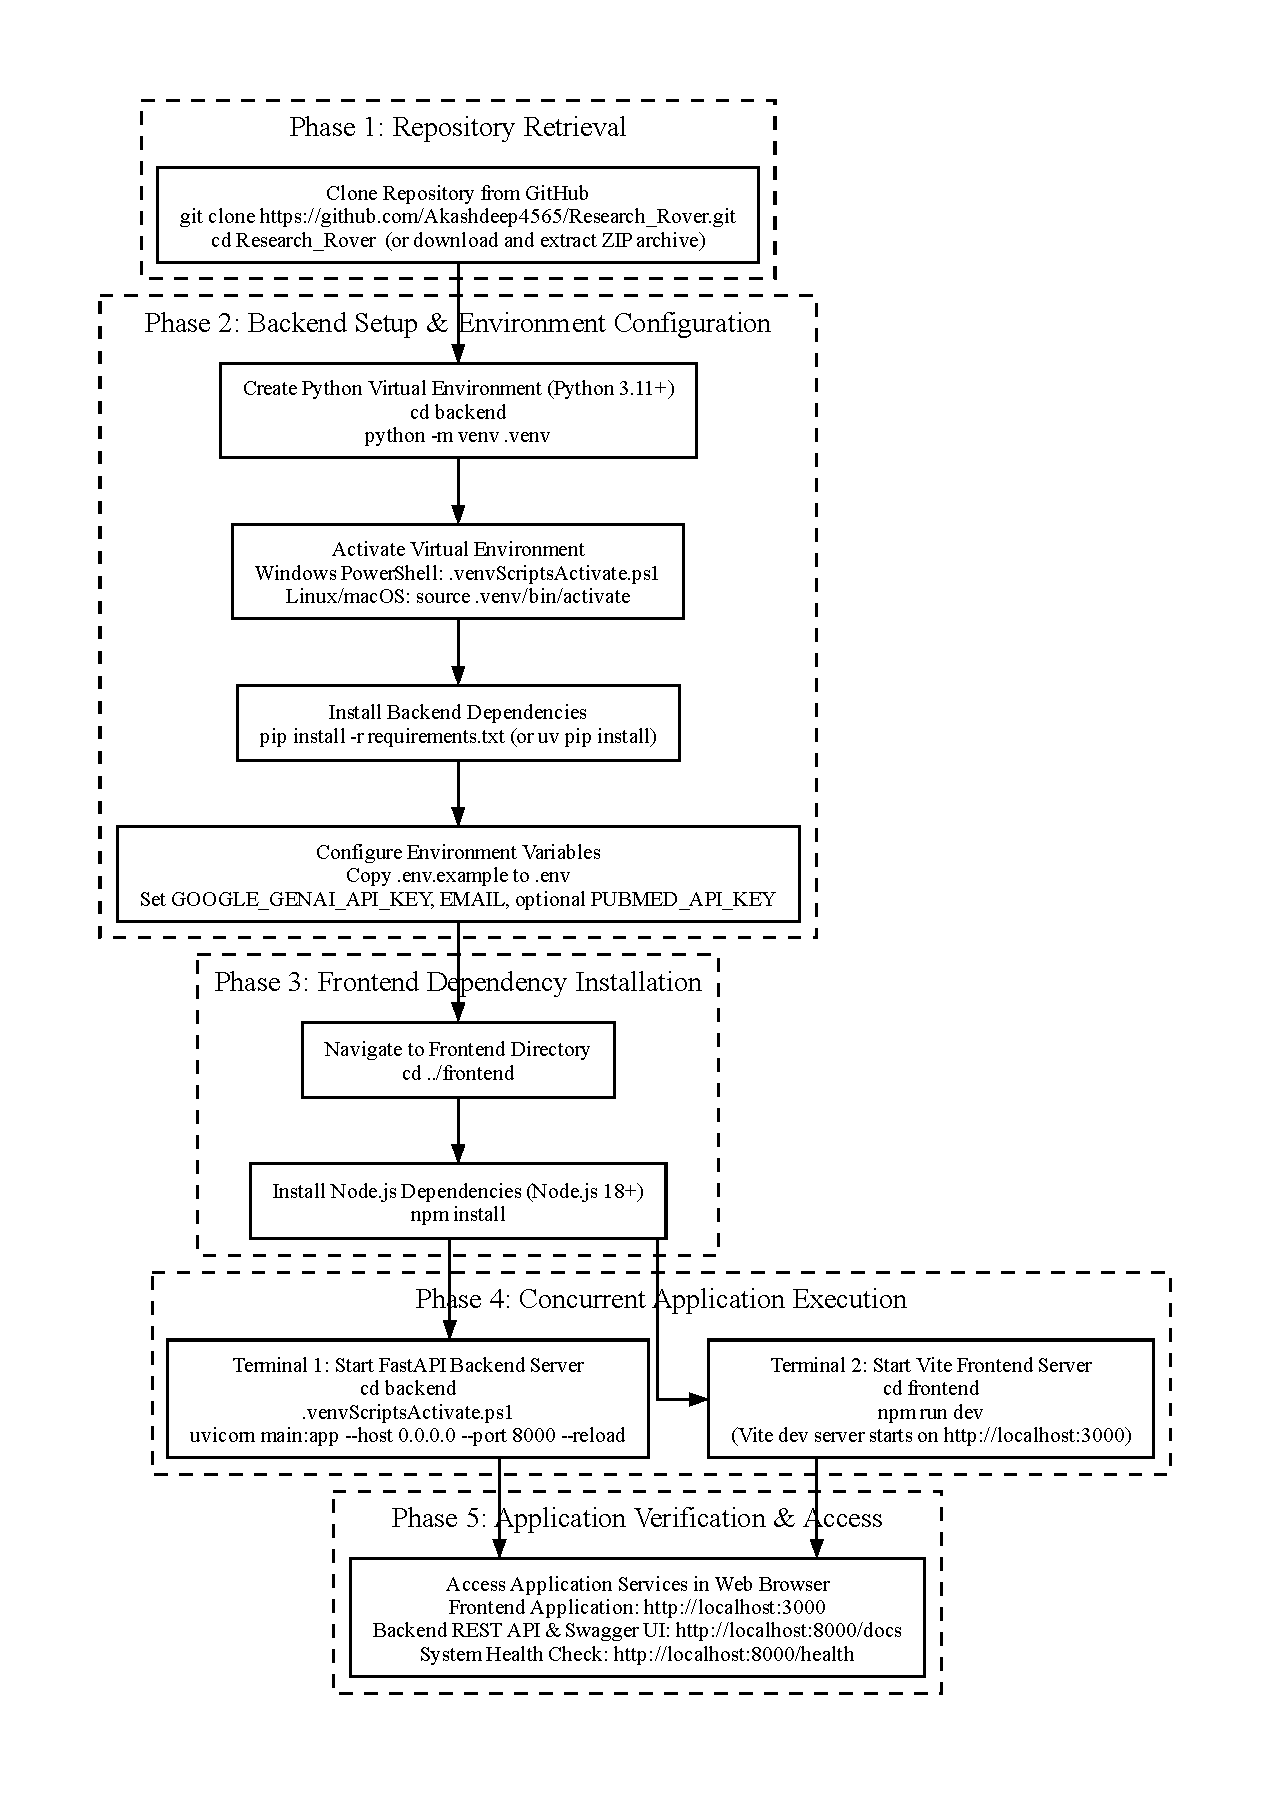
\includegraphics[width=0.88\textwidth]{figures/installation_workflow.pdf}
\caption{End-to-End Installation, Configuration, and Execution Workflow}
\label{fig:installation_workflow}
\end{figure}

Figure~\ref{fig:installation_workflow} illustrates the end-to-end procedural workflow required to set up both backend and frontend environments.

\subsection{Backend Installation and Environment Setup}
The backend application is encapsulated within the \texttt{backend/} directory. All dependency installations should be isolated within a dedicated Python virtual environment.

\subsubsection{Step 1: Create and Activate Python Virtual Environment}
Navigate to the \texttt{backend} subdirectory:

\begin{lstlisting}[language=bash, caption={Creating and Activating Virtual Environment}]
# Navigate to backend directory
cd backend

# Create isolated virtual environment named .venv
python -m venv .venv

# Activate on Windows PowerShell:
.venv\Scripts\Activate.ps1

# Activate on Windows Command Prompt (cmd.exe):
.venv\Scripts\activate.bat

# Activate on macOS / Linux:
source .venv/bin/activate
\end{lstlisting}

\noindent \textit{PowerShell Execution Policy Note:} If Windows PowerShell returns a script execution policy error (\texttt{PSSecurityException}), permit local script execution by running:
\begin{lstlisting}[language=powershell]
Set-ExecutionPolicy -ExecutionPolicy RemoteSigned -Scope CurrentUser
\end{lstlisting}

\subsubsection{Step 2: Install Backend Python Dependencies}
Ensure \texttt{pip} is upgraded to the latest version, then install all pinned dependencies from \texttt{requirements.txt}:

\begin{lstlisting}[language=bash, caption={Installing Backend Python Packages}]
python -m pip install --upgrade pip
pip install -r requirements.txt
\end{lstlisting}

\noindent The installation encompasses key packages including \texttt{fastapi==0.115.6}, \texttt{uvicorn==0.34.0}, \texttt{torch==2.7.0}, \texttt{transformers==4.52.2}, \texttt{sentence-transformers==4.1.0}, \texttt{faiss-cpu==1.11.0}, \texttt{google-generativeai==0.8.5}, \texttt{Crawl4AI==0.6.3}, and \texttt{pandas==2.2.3}.

\subsubsection{Step 3: Configure Backend Environment Variables}
The backend relies on environment variables defined in a \texttt{.env} file located at \texttt{backend/.env}. A reference template is provided in \texttt{backend/.env.example}. Copy the template:

\begin{lstlisting}[language=bash, caption={Initializing Environment Configuration}]
# On Windows PowerShell:
Copy-Item .env.example .env

# On macOS / Linux:
cp .env.example .env
\end{lstlisting}

Open \texttt{backend/.env} in a text editor and populate the verified configuration values:

\begin{lstlisting}[caption={Example backend/.env Configuration File}]
# Mandatory: Google Gemini API Key for Chat & RAG
GOOGLE_GENAI_API_KEY="AIzaSyYourActualGeminiApiKeyGoesHere"

# Mandatory: Valid email address for NCBI PubMed API etiquette
EMAIL="researcher@university.edu"

# Optional: Personal NCBI PubMed API Key (increases rate limit to 10 req/s)
PUBMED_API_KEY=""

# Optional: OpenAlex API key for high-throughput scholarly search
OPENALEX_API_KEY=""
\end{lstlisting}

\subsection{Frontend Installation and Setup}
The frontend user interface is contained in the \texttt{frontend/} directory and is managed via Node.js and npm.

\subsubsection{Step 1: Navigate and Install Node Dependencies}
Open a new terminal window or navigate out of the backend directory into \texttt{frontend}:

\begin{lstlisting}[language=bash, caption={Installing Frontend Dependencies}]
cd ../frontend
npm install
\end{lstlisting}

\noindent This installs all packages specified in \texttt{package.json}, including React 19, Vite 6, Tailwind CSS, Lucide icons, Three.js, and Radix UI components.

\subsubsection{Step 2: Verify Vite Development Server Configuration}
The frontend development server configuration is defined in \texttt{frontend/vite.config.ts}:

\begin{lstlisting}[language=javascript, caption={Vite Server Port and Reverse Proxy in vite.config.ts}]
export default defineConfig({
  plugins: [react()],
  resolve: {
    alias: {
      "@": path.resolve(__dirname, "./src"),
    },
  },
  server: {
    port: 3000,
    proxy: {
      '/api': {
        target: 'http://localhost:8000',
        changeOrigin: true,
      },
    },
  },
})
\end{lstlisting}

\noindent As configured, the Vite dev server binds to port \textbf{3000} and automatically proxies all API requests beginning with \texttt{/api} to the FastAPI backend running on \texttt{http://localhost:8000}.
